\documentclass[12pt]{article}
\usepackage[utf8]{inputenc}
\newcommand\preamble{
    \usepackage[italian]{babel}
    \usepackage{geometry}
    \usepackage{amsmath}
    \usepackage{amssymb}
    \usepackage{graphicx}
    \usepackage{ulem}
    \usepackage[dvipsnames]{xcolor}

    \geometry{margin=2cm}
    \let\olditemize\itemize
    \renewcommand\itemize{\olditemize\setlength\itemsep{0em}}
    \graphicspath{{../Immagini/}}

    \author{Lorenzo Vaccarecci}
}
\preamble

\title{Ottimizzazione Logica}
\date{19 Aprile 2024}

\begin{document}
\maketitle
\section{Introduzione}
\begin{itemize}
    \item \textbf{Input:} espressione algebrica
    \item \textbf{Output:} piano di esecuzione logico ottimizzato (LQP)
\end{itemize}
\textcolor{red}{Piano di esecuzione logico}: espressione algebrica per l'interrogazione rappresentata come albero
\begin{center}
    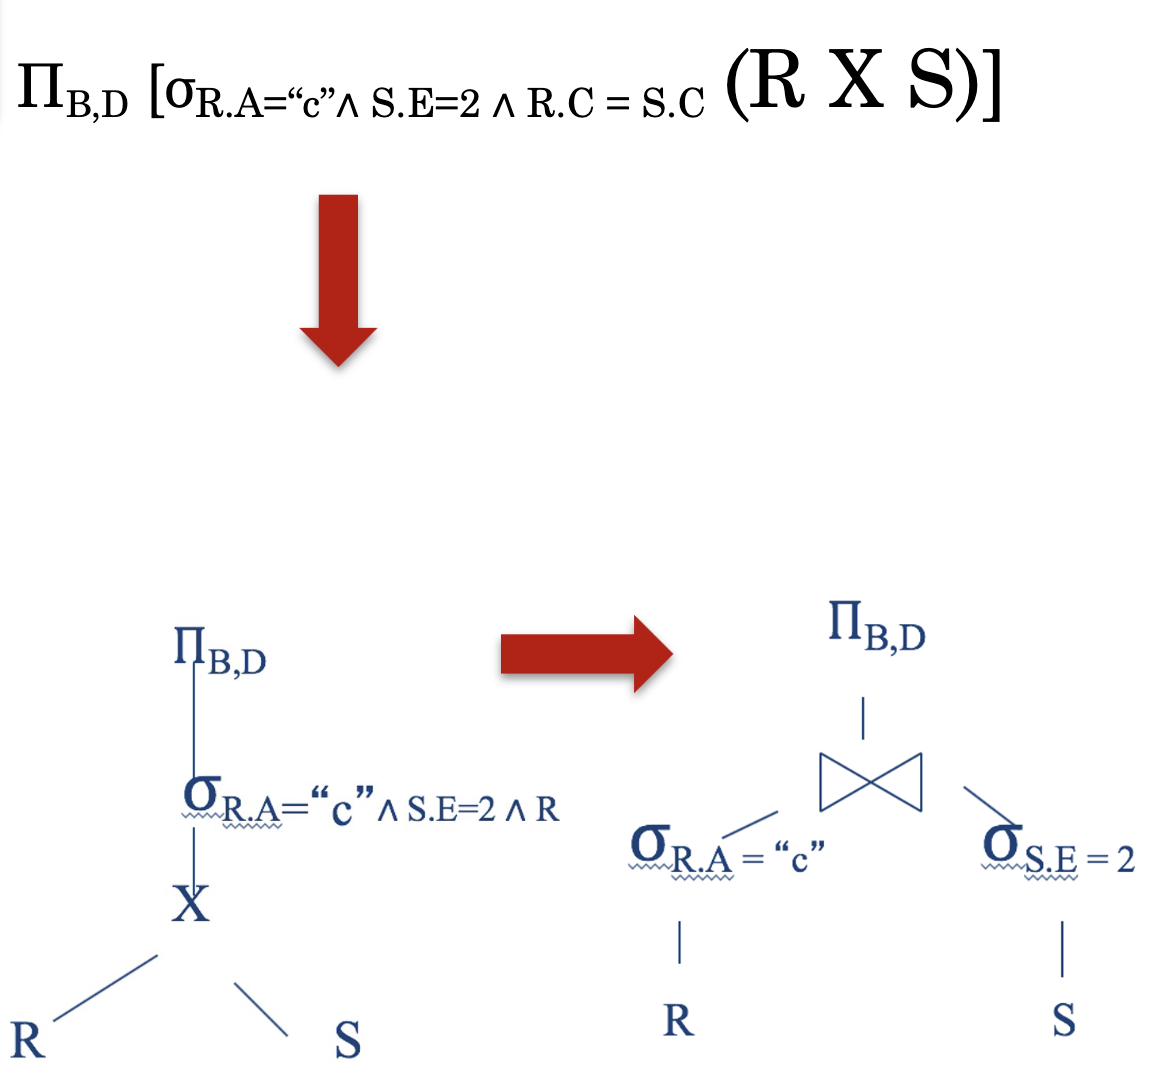
\includegraphics[scale=0.4]{esempioalberologicoottimizzato.png}*
\end{center}
\textit{*L'esempio è incompleto ma rende l'idea}\\
Per ottimizzare l'albero, sfrutta le proprietà dell'algebra relazionale
\section{Come avviene l'ottimizzazione}
\begin{itemize}
    \item si basa su \textcolor{red}{equivalenze algebriche} \begin{itemize}
        \item si dicono equivalenti se $e_{1}$ e $e_{2}$ restituiscono lo \textbf{stesso risultato}
    \end{itemize}
    \item queste equivalenze sono usate come \textcolor{red}{regole di riscrittura}, utilizzando opportune \textcolor{red}{euristiche} per passare da una espressione algebrica a un'altra
\end{itemize}
Regola di riscrittura: posso sostituire $e_{1}$ con $e_{2}$ se valgono determinate condizioni $C$.\\
Nell'ottimizzazione logica la regola verrà considerata se $e_{2}$ è "efficiente" 
\subsection{Esempi notevoli (da ricordare)}
\textit{Altri esempi sulle slide, queste sono le principali}
\subsubsection{Selezione}
\begin{equation*}
    \sigma_{P1}(\sigma_{P2}(e))\equiv \sigma_{P2}(\sigma_{P1}(e)) \equiv \sigma_{P1 \land P2}(e)
\end{equation*}
\subsubsection{Proiezione}
\begin{equation*}
    \Pi_{A1,\ldots,An}(\Pi_{B1,\ldots,Bn}(e))\equiv \Pi_{A1,\ldots,An}(e)
\end{equation*}
\begin{itemize}
    \item Permette di gestire cascate di proiezioni
    \item vale se $\left\{A1,\ldots,An\right\}\subseteq \left\{B1,\ldots,Bn\right\}$
\end{itemize}
\subsubsection{Commutazione di selezione e proiezione}
\begin{equation*}
    \Pi_{A1,\ldots,An}(\sigma_{P}(e))\equiv \sigma_{P}(\Pi_{A1,\ldots,An}(e))
\end{equation*}
Vale solo se $P \subseteq \left\{A1,\ldots,An\right\}$
\subsubsection{Commutazione di selezione e prodotto cartesiano}
\begin{equation*}
    \sigma_{P}(e_{1}\times e_{2}) \equiv \sigma_{P}(e_{1})\times e_{2}
\end{equation*}
Vale solo se $P$ coinvolge gli attributi di $e_{1}$
\subsubsection{Commutazione di proiezione e prodotto cartesiano}
\begin{equation*}
    \Pi_{A1,\ldots,An}(e_{1}\times e_{2})\equiv \Pi_{B1,\ldots,Bn}(e_{1}) \times \Pi_{C1,\ldots,Cn}(e_{2})
\end{equation*}
\subsubsection{Selezioni, prodotto cartesiano e join}
\begin{equation*}
    \sigma_{P}(e_{1} \times e_{2}) \equiv e_{1}\Join_{P}  e_{2}
\end{equation*}
\subsubsection{Prodotto cartesiano e join (Slide 34) \textcolor{red}{Da completare}}
\begin{itemize}
    \item \textbf{Commutatività} \begin{itemize}
        \item $e_{1} \Join_{F} e_{2} \equiv e_{2} \Join_{F} e_{1}$
        \item $e_{1} \Join e_{2} \equiv e_{2} \Join e_{1}$
        \item $e_{1} \times e_{2} \equiv e_{2} \times e_{1}$
    \end{itemize}
    \item \textbf{Associatività} \begin{itemize}
        \item 
    \end{itemize}
\end{itemize}
\subsubsection{Unione e differenza (Slide 35) \textcolor{red}{Da completare}}
\begin{itemize}
    \item \textbf{Commutatività}
    \item \textbf{Associatività}
\end{itemize}
\section{Euristiche}
Le \textcolor{red}{euristiche} permettono di trasformare le equivalenze in
regole di riscrittura. Va un po' a "buon senso", guarda quale delle riscritture ha l'input minore.
\subsection{Euristiche fondamentali}
\begin{itemize}
    \item anticipare il più possibile \textbf{selezioni} e \textbf{proiezioni}
    \item fattorizzare condizioni di selezione complesse per aumentare la possibilità di applicare le regole di riscrittura
\end{itemize}
\subsection{Euristiche principali}
\textcolor{red}{Nessuna regola di riscrittura si riferisce all’ordine con cui
eseguire un insieme di join (verrà ottimizzato al livello fisico).}
\begin{itemize}
    \item \textbf{1A}: eseguire le operazioni di selezione il più presto possibile
    \item \textbf{1B}: eseguire le operazioni di proiezione il più presto possibile
    \item \textbf{2}: fattorizzare condizioni di selezione complesse per aumentare la possibilità di applicare le regole di riscrittura (come ad esempio 2.1.1)
\end{itemize}
\subsubsection{Esempio}
Relazioni: $R(ABC) \quad S(DEF)$ \\
Query: $\Pi_{BE}(\sigma_{A>5\land F>6 \land C=D}(R\times S))$\\
\textit{Ottimizzazione:}
\begin{description}
    \item[$\rightarrow^{1A}$] $\Pi_{BE}(\sigma_{C=D}(\sigma_{A>5}(\sigma_{F>6}(R\times S))))$
    \item[$\rightarrow^{1A}$] $\Pi_{BE}(\sigma_{C=D}(\sigma_{A>5}(R\times \sigma_{F>6}(S))))$
    \item[$\rightarrow^{1A}$] $\Pi_{BE}(\sigma_{C=D}(\sigma_{A>5}(R)\times \sigma_{F>6}(S)))$
\end{description}
\section{Output}
\textcolor{red}{L’output della fase di ottimizzazione logica è un singolo LQP ottimizzato}. Si potrebbe anche guardare LQP alternativi ma non viene utilizzata perchè per ognuno bisognerebbe individuarne il piano fisico ottimale.
\end{document}